\documentclass[../report.tex]{subfiles}
\begin{document}
\subsection{Mạng liên kết là gì ?}   
\paragraph*{}Mạng liên kết là một hệ thống vận chuyển dữ liệu có thể lập trình được giữa các thiết bị đầu cuối (terminal). Hình vẽ thể hiện một mạng liên kết, trong đó có 6 termial, T1 tới T6, được kết nối với mạng. Khi terminal T3 muốn trao đổi dữ liệu với terminal T5, nó sẽ gửi một tin nhắn có chứa dữ liệu vào trong mạng và mạng sẽ làm nhiệm vụ vận chuyển tin nhắn tới T5. Mạng có thể lập trình được theo nghĩa nó có thể tạo kết nối với nhiều điểm khác nhau tại cùng một thời điểm. Mạng biểu diễn trong hình có thể chuyển tin nhẵn từ T3 tới T5 trong một chu kì và sau đó sử dụng cùng tài nguyên đó để chuyển một tin nhẵn mới từ T3 tới T1 trong chu kì tiếp theo. Mạng liên kết được coi là một hệ thống bởi nó bao gồm nhiều thành phần: buffer, channel, switch và control, các thành phần này làm việc cùng nhau để hoàn thành nhiệm vụ chính đó là vận chuyển dữ liệu.
\begin{figure}[H]
\centering
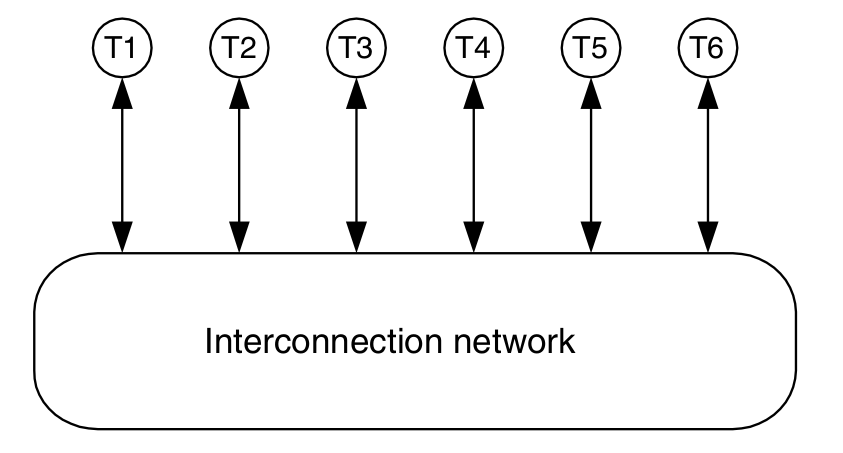
\includegraphics[width=9cm]{figures/interconnection.png}
\caption{Góc nhìn chức năng của một mạng liên kết. Terminals (được gán nhãn T1 tới T6) được kế nối với mạng sử dụng channels}
\end{figure}

\subsection{Mạng liên kết được dùng ở đâu ?}
\paragraph*{} Hầu hết các hệ thống số lớn (các hệ thống có nhiều thành phần cần trao đổi dữ liệu với nhau) đều có sử dụng mạng liên kết. Ứng dụng phổ biến của mạng liên kết đó là trong các hệ thống máy tính và giao tiếp giữa các switch. Trong hệ thống máy tính, chúng kết nối processor với bộ nhớ và thiết bị nhập xuất với bộ điều khiển nhập xuất. Chúng kết nối các cổng vào với các cổng ra trong giao tiếp với switch và với processor trong hệ thống điều khiển. Bất hệ thống nào xuất hiện sự trao đổi dữ liệu giữa hai hay nhiều thành phần của nó với nhau thì hệ thống có sử dụng tới mạng liên kết.

\subsection{Vai trò của mạng liên kết}
\paragraph*{}Hiện tay, mạng liên kết được ứng dụng rộng rãi trong các hệ thống máy tính và các hệ thống chuyển mạch thông tin liên lạc. Đặc biệt mạng liên được thiết kế sử dụng ở các mức độ khác nhau trong các hệ thống máy tính nhằm đáp ứng nhu cầu của các nhóm ứng dụng khác nhau như: tính toán hiệu năng cao, tính toán phân tán, \ldots Tùy thuộc vào số lượng các thiết bị được kết nối và khoảng cách giữa các thiết bị, mạng liên kết được chia ra làm bốn lĩnh vực ứng dụng chính:
\begin{itemize}
    \item On-chip networks (OCNs) hay còn được nhắc tới với thuật ngữ network-on-chip (NoC): được sử dụng để kết nối bên trong các vi kiến trúc giữa các đơn vị chức năng, thanh ghi (register), bộ lưu trữ trung gian (caches), các bộ vi xử lý (processor) trong các module đa chip. OCNs hỗ trợ các kết nối giữa vài chục thiết bị đặt trong các vi mạch với khoảng cách tối đa khoảng vài centimet.
    \item System/storage area networks (SANs): Đây là mạng liên kết được sử dụng để kết nối các bộ vi xử lý liên kết (interprocessor) và các bộ nhớ (processor-memory) trong các hệ thống đa nhân và hệ thống đa máy tính (multicomputer). Ngoài ra loại mạng liên kết này cũng được sử dụng để kết nối các thành phần lưu trữ và thành phần xử lý vào ra trong môi trường gồm các máy chủ (server) và các trung tâm dữ liệu (data centers). Số lượng thiết bị được kết nối trong SANs có thể lên tới hàng nghìn thiết bị khác nhau phân bố với khoảng cách khoảng vài trăm met
    \item Local area networks (LANs): Đây là mạng liên kết được sử dụng để kết nối hệ thống máy tính cá nhân. Kết nối máy tính trong một cụm là một ví dụ điển hình. Ban đầu, các mạng LAN chỉ kết nối hàng trăm thiết bị, nhưng với cầu nối (bridges), mạng LAN có thể kết nối lên đến vài nghìn thiết bị. Khoảng cách kết nối tối đa bao phủ khu vực có đường kính vài kilomet đến vài chục kilomet.
    \item Wide area networks (WANs): WANs kết nối các hệ thống máy tính phân bố phân tán trên toàn thế giới. WANs cũng kết nối hàng triệu các máy tính với nhau trên khoảng cách lớn.
\end{itemize}
\end{document}
